\documentclass[a4paper,12pt]{article}

\usepackage[portuguese]{babel}
\usepackage[utf8]{inputenc}
\usepackage{graphics}
\usepackage {color}
\usepackage{graphicx}
\usepackage{geometry}
\usepackage{flushend}
\usepackage[normalem]{ulem}              % para sublinhar texto
\usepackage{fancyhdr}                    % Para cabeçalhos
\usepackage{url}                         % Para tratar endereços 'url'
\usepackage{kpfonts}
\usepackage{latexsym}
\usepackage{hyperref}                 % For creating hyperlinks in cross references
\usepackage{amssymb}           % carrega letras matemáticas

\title{A vida do Suricata}
\author{Omeir Haroon}
\date {\today}


\begin{document}
\maketitle
\section{Sobre o Saricato}
O suricata, também chamado de \textbf{suricato ou suricate} (Suricata suricatta) é um pequeno mamífero da família Herpestidae, nativo do deserto do Kalahari. Estes animais têm cerca de meio metro de comprimento (incluindo a cauda), em média 730 gramas de peso, e pelagem acastanhada. Têm garras afiadas nas patas, que lhes permitem escavar a superfície do chão e dentes afiados para penetrar nas carapaças quitinosas das suas presas. Outra característica distinta é a sua capacidade de se elevarem nas patas traseiras, utilizando a cauda como terceiro apoio. 

\section{Caracteristicas gerais}
\subsection{Alimentacao}
Alimenta-se principalmente de insetos (cerca de 82 \%): larvas de escaravelhos e de borboletas; também ingerem milípedes, aranhas, escorpiões, pequenos vertebrados (répteis, anfíbios e aves), ovos e matéria vegetal. São relativamente imunes ao veneno das najas e dos escorpiões, sendo estes, inclusive, um dos alimentos que mais apreciam.

\begin{figure}
   \caption{Suricata no Zoo de Lisboa}
   \centering
   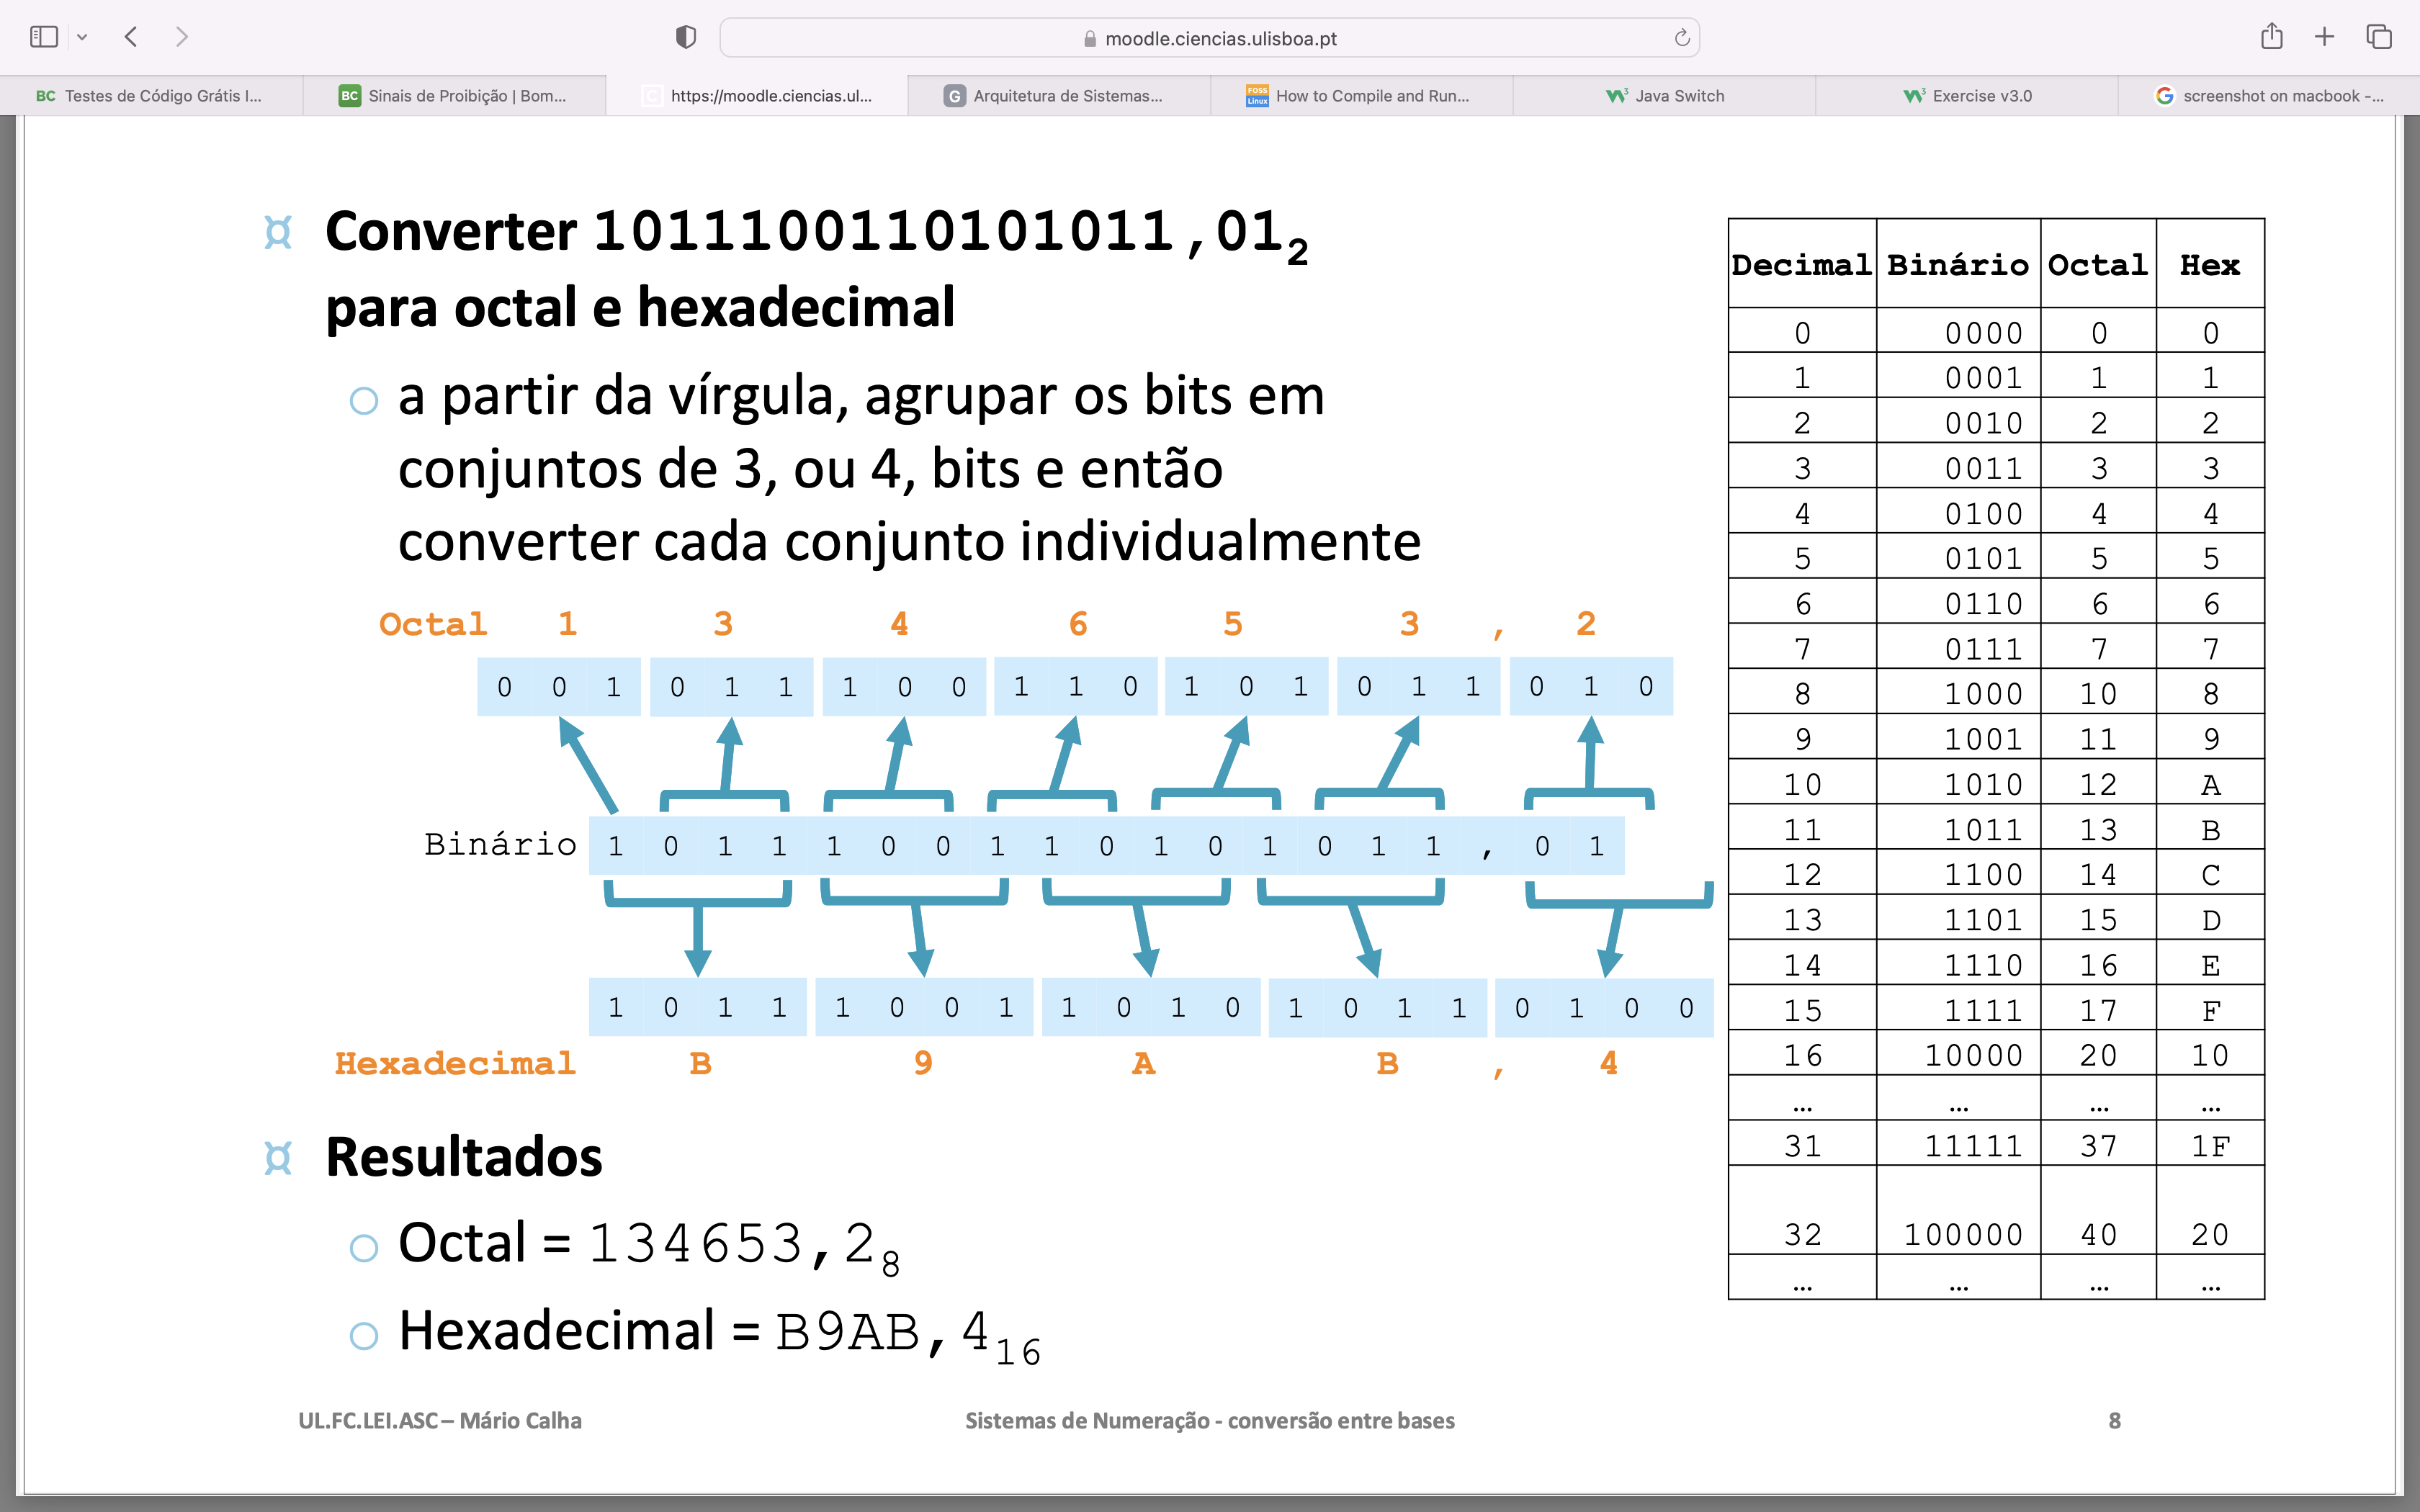
\includegraphics[scale=0.38]{image}
   \end{figure}

\end{document}